\subsection{Passage à l'échelle}
\label{sec:compteur}
Comme dit dans le chapitre précédent, l'algorithme du GMRES se parallélise bien parce qu'il est essentiellement composé d'opérations sur des vecteurs.
%
L'opération la plus coûteuse est le produit d'une matrice par un vecteur (SpMV).
%
Notre implémentation du SpMV est optimisée pour prendre en compte la structure bloc des entrées de la matrice quand le nombre de variables primaires est supérieur à 1.
%
Nos matrices sont stockées au format BCSR, les éléments contenus dans les petits blocs denses sont contigus en mémoire.
%
Cela nous permet d'optimiser les effets caches et nous pouvons aussi utiliser le jeu d'instructions vectorielles de nos processeurs.

Malgré les optimisations des effets caches, le SpMV est toujours limité par la bande passante mémoire.
%
Les courbes d'accélération du SpMV nous montrent que le gain de performance n'est pas linéaire avec le nombre de coeurs (Fig.~\ref{fig:res_spmv_omp_rostand}).
%
Le constat est même pire que ça, on arrive difficilement à une accélération de 2 sur 12 coeurs lorsqu'on utilise une seule variable primaire.
%   (-_-)   %
\begin{figure}[!h]
  \centering
  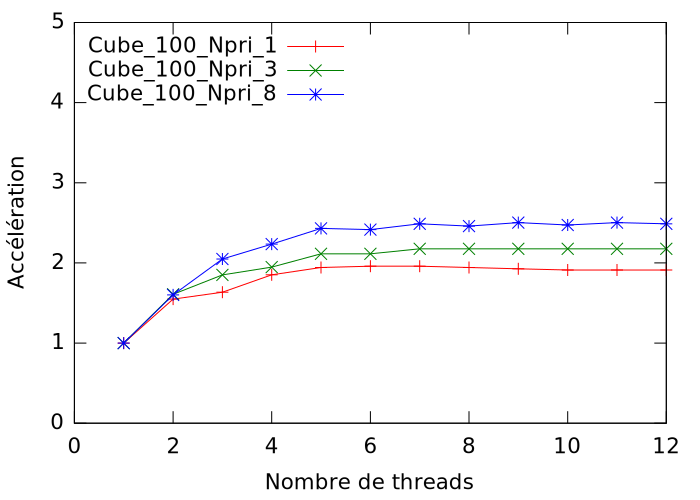
\includegraphics[width=0.7\textwidth]{res_spmv_omp}
  \caption{Accélération du produit matrice vecteur creux sur Rostand en mémoire partagée.}
  \label{fig:res_spmv_omp_rostand}
\end{figure}

Pour comprendre ce qui se passe, nous allons utiliser les compteurs matériels de la machine.
%
Ces compteurs sont intégrés au processeur et on y accède via des registres spéciaux seulement disponibles en espace noyau.
%
De nombreux logiciels proposent une interface d'accès à ces compteurs, mais certains nécessitent le chargement d'un module noyau.


Linux propose un outil d'analyse de performance natif nommé {\em perf}.
%
Cet outil se présente sous la forme d'un exécutable qui se lance juste avant notre programme.
%
Nous devons choisir nous même les compteurs qui nous intéressent.
%
Malheureusement, la version du noyau Linux installé sur nos machines ne nous permet pas d'accéder à tous les compteurs.
%
Il manque essentiellement les compteurs de type {\em uncore} qui permettent de mesurer le nombre de requêtes mémoire faites à un banc NUMA distant.




PAPI\footnote{Performance Application Programming Interface} est une interface de programmation qui fournit une abstraction pour l'accès aux compteurs matériels.
%
Cette bibliothèque utilise l'interface perfmon sous Linux, elle utilise donc le même module noyau que perf.
%
En plus de faciliter l'accès aux compteurs, elle propose comme fonctionnalité de simuler des accumulateurs de compteurs.
%
Mais son mode de fonctionnement dans un environnement multi-threadé n'est pas suffisamment documenté.



Intel propose aussi un outil d'analyse de performances, il s'agit de Intel VTune.
%
Cet outil est hautement configurable avec des profils prédéfinis.
%
L'exécution du code échantillonnée avec les valeurs des compteurs matériels associés à chaque échantillon.
%
Cet outil est très complet, mais requiert l'achat d'une licence d'utilisation ainsi que l'ajout d'un module noyau.
%
Nous n'avons donc pas pu utiliser cet outil car les administrateurs de notre grappe de serveur ont refusés d'installer le module noyau.



Nous avons préféré utiliser Likwid, un outil d'analyse de performance léger qui simplifie l'accès aux compteurs matériels.
%
Le principal avantage de Likwid est qu'il contient des profils déjà configurés calculant des métriques 
%
Par exemple, le profil {\em MEM} nous donnera directement les mesures de bande passante mémoire locale et distante en divisant le nombre d'accès mémoire par le temps de calcul.
%
Le nombre d'accès mémoire provient des compteurs {\em UNC\_QMC\_NORMAL\_READS\_ANY}, {\em UNC\_QMC\_WRITES\_FULL\_ANY}, {\em UNC\_QHL\_REQUESTS\_REMOTE\_READS} et {\em UNC\_QHL\_REQUESTS\_REMOTE\_WRITES}.
%
Il y a aussi la possibilité d'interagir avec Likwid depuis le code d'une application pour ne mesurer qu'une portion du code.
%
Nous utiliserons cette fonctionnalité pour ne mesurer que la routine qui nous intéresse.



Pour mesurer les effets NUMA sur le SpMV, nous effectuons 100 SpMV et mesurerons le nombre d'accès mémoire.
%
Si l'on regarde les compteurs matériels (Table~\ref{tab:numa_spmv}), on s'aperçoit que la moitié de la bande passante en lecture de chaque banc NUMA est utilisée par des accès distants.
%
Donc environ la moitié des lectures mémoires sont faites avec une plus grande latence.
%
Nous pouvons aussi remarquer un déséquilibre de charge.
%
Le thread responsable de l'initialisation du code s'est exécuté sur le banc NUMA 1.
%
Les pages mémoires servant à stocker la matrice étaient donc quasiment toutes sur ce banc NUMA.

%   (-_-)   %
\begin{center}
  \begin{tabular}{|r|c|c|c|c|}
    \hline
                & Lecture locale & Lecture distante & \'Ecriture locale & \'Ecriture distante \\
    \hline
    Banc NUMA 0 & 8,68E+07  &  9,18E+07  &  6,24E+07  &  2,29E+07 \\
    Banc NUMA 1 & 4,08E+09  &  2,60E+09  &  2,68E+08  &  5,64E+07 \\
    \hline
  \end{tabular}
  \captionof{table}{Nombre d'accès mémoire effectués lors de 100 produits matrice vecteur creux.}
  \label{tab:numa_spmv}
\end{center}
